\documentclass[twoside]{book}

% Packages required by doxygen
\usepackage{fixltx2e}
\usepackage{calc}
\usepackage{doxygen}
\usepackage[export]{adjustbox} % also loads graphicx
\usepackage{graphicx}
\usepackage[utf8]{inputenc}
\usepackage{makeidx}
\usepackage{multicol}
\usepackage{multirow}
\PassOptionsToPackage{warn}{textcomp}
\usepackage{textcomp}
\usepackage[nointegrals]{wasysym}
\usepackage[table]{xcolor}

% Font selection
\usepackage[T1]{fontenc}
\usepackage[scaled=.90]{helvet}
\usepackage{courier}
\usepackage{amssymb}
\usepackage{sectsty}
\renewcommand{\familydefault}{\sfdefault}
\allsectionsfont{%
  \fontseries{bc}\selectfont%
  \color{darkgray}%
}
\renewcommand{\DoxyLabelFont}{%
  \fontseries{bc}\selectfont%
  \color{darkgray}%
}
\newcommand{\+}{\discretionary{\mbox{\scriptsize$\hookleftarrow$}}{}{}}

% Page & text layout
\usepackage{geometry}
\geometry{%
  a4paper,%
  top=2.5cm,%
  bottom=2.5cm,%
  left=2.5cm,%
  right=2.5cm%
}
\tolerance=750
\hfuzz=15pt
\hbadness=750
\setlength{\emergencystretch}{15pt}
\setlength{\parindent}{0cm}
\setlength{\parskip}{3ex plus 2ex minus 2ex}
\makeatletter
\renewcommand{\paragraph}{%
  \@startsection{paragraph}{4}{0ex}{-1.0ex}{1.0ex}{%
    \normalfont\normalsize\bfseries\SS@parafont%
  }%
}
\renewcommand{\subparagraph}{%
  \@startsection{subparagraph}{5}{0ex}{-1.0ex}{1.0ex}{%
    \normalfont\normalsize\bfseries\SS@subparafont%
  }%
}
\makeatother

% Headers & footers
\usepackage{fancyhdr}
\pagestyle{fancyplain}
\fancyhead[LE]{\fancyplain{}{\bfseries\thepage}}
\fancyhead[CE]{\fancyplain{}{}}
\fancyhead[RE]{\fancyplain{}{\bfseries\leftmark}}
\fancyhead[LO]{\fancyplain{}{\bfseries\rightmark}}
\fancyhead[CO]{\fancyplain{}{}}
\fancyhead[RO]{\fancyplain{}{\bfseries\thepage}}
\fancyfoot[LE]{\fancyplain{}{}}
\fancyfoot[CE]{\fancyplain{}{}}
\fancyfoot[RE]{\fancyplain{}{\bfseries\scriptsize Generated by Doxygen }}
\fancyfoot[LO]{\fancyplain{}{\bfseries\scriptsize Generated by Doxygen }}
\fancyfoot[CO]{\fancyplain{}{}}
\fancyfoot[RO]{\fancyplain{}{}}
\renewcommand{\footrulewidth}{0.4pt}
\renewcommand{\chaptermark}[1]{%
  \markboth{#1}{}%
}
\renewcommand{\sectionmark}[1]{%
  \markright{\thesection\ #1}%
}

% Indices & bibliography
\usepackage{natbib}
\usepackage[titles]{tocloft}
\setcounter{tocdepth}{3}
\setcounter{secnumdepth}{5}
\makeindex

% Hyperlinks (required, but should be loaded last)
\usepackage{ifpdf}
\ifpdf
  \usepackage[pdftex,pagebackref=true]{hyperref}
\else
  \usepackage[ps2pdf,pagebackref=true]{hyperref}
\fi
\hypersetup{%
  colorlinks=true,%
  linkcolor=blue,%
  citecolor=blue,%
  unicode%
}

% Custom commands
\newcommand{\clearemptydoublepage}{%
  \newpage{\pagestyle{empty}\cleardoublepage}%
}

\usepackage{caption}
\captionsetup{labelsep=space,justification=centering,font={bf},singlelinecheck=off,skip=4pt,position=top}

%===== C O N T E N T S =====

\begin{document}

% Titlepage & ToC
\hypersetup{pageanchor=false,
             bookmarksnumbered=true,
             pdfencoding=unicode
            }
\pagenumbering{alph}
\begin{titlepage}
\vspace*{7cm}
\begin{center}%
{\Large Infotheory \\[1ex]\large 1.\+0 }\\
\vspace*{1cm}
{\large Generated by Doxygen 1.8.14}\\
\end{center}
\end{titlepage}
\clearemptydoublepage
\pagenumbering{roman}
\tableofcontents
\clearemptydoublepage
\pagenumbering{arabic}
\hypersetup{pageanchor=true}

%--- Begin generated contents ---
\chapter{Hierarchical Index}
\section{Class Hierarchy}
This inheritance list is sorted roughly, but not completely, alphabetically\+:\begin{DoxyCompactList}
\item object\begin{DoxyCompactList}
\item \contentsline{section}{infotheory.\+infotools.\+Info\+Tools}{\pageref{classinfotheory_1_1infotools_1_1_info_tools}}{}
\end{DoxyCompactList}
\end{DoxyCompactList}

\chapter{Class Index}
\section{Class List}
Here are the classes, structs, unions and interfaces with brief descriptions\+:\begin{DoxyCompactList}
\item\contentsline{section}{\mbox{\hyperlink{class_info_tools}{Info\+Tools}} }{\pageref{class_info_tools}}{}
\end{DoxyCompactList}

\chapter{Class Documentation}
\hypertarget{classinfotheory_1_1infotools_1_1_info_tools}{}\section{infotheory.\+infotools.\+Info\+Tools Class Reference}
\label{classinfotheory_1_1infotools_1_1_info_tools}\index{infotheory.\+infotools.\+Info\+Tools@{infotheory.\+infotools.\+Info\+Tools}}
Inheritance diagram for infotheory.\+infotools.\+Info\+Tools\+:\begin{figure}[H]
\begin{center}
\leavevmode
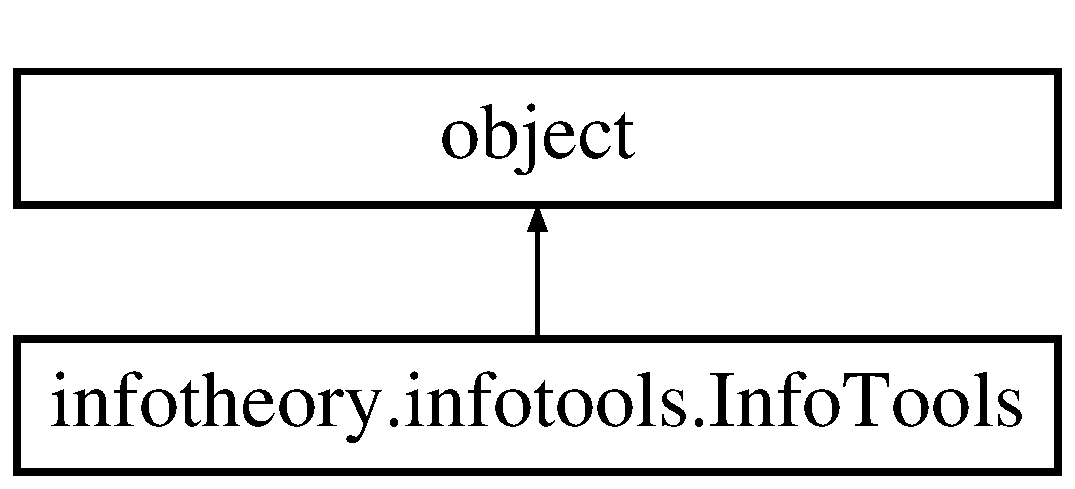
\includegraphics[height=2.000000cm]{classinfotheory_1_1infotools_1_1_info_tools}
\end{center}
\end{figure}
\subsection*{Public Member Functions}
\begin{DoxyCompactItemize}
\item 
def \mbox{\hyperlink{classinfotheory_1_1infotools_1_1_info_tools_aee293b361cf0511b521fbdc88a3e4d15}{\+\_\+\+\_\+init\+\_\+\+\_\+}} (self, dims, nreps, nbins, mins, maxs)
\item 
def \mbox{\hyperlink{classinfotheory_1_1infotools_1_1_info_tools_a56f38bf629e7a7831f3d0ee738df1077}{add\+\_\+data\+\_\+point}} (self, datapoint)
\item 
def \mbox{\hyperlink{classinfotheory_1_1infotools_1_1_info_tools_a7a424c5612b0bd7f9e06358283bab828}{add\+\_\+data}} (self, data)
\item 
def \mbox{\hyperlink{classinfotheory_1_1infotools_1_1_info_tools_ab869cf9c1cfa0462dba819a52d040304}{clear\+All\+Data}} (self)
\item 
def \mbox{\hyperlink{classinfotheory_1_1infotools_1_1_info_tools_a702d0595303876470eec677c2d3807c8}{\+\_\+\+\_\+del\+\_\+\+\_\+}} (self)
\item 
def \mbox{\hyperlink{classinfotheory_1_1infotools_1_1_info_tools_afe2bba77e05df1103d38261748772a18}{entropy}} (self, var\+\_\+\+I\+Ds)
\item 
def \mbox{\hyperlink{classinfotheory_1_1infotools_1_1_info_tools_a77f444a7cba9457f8bf30c9e2d02ea86}{mutual\+\_\+info}} (self, var\+\_\+\+I\+Ds)
\item 
def \mbox{\hyperlink{classinfotheory_1_1infotools_1_1_info_tools_a865054984e7894a8e4852f6ac26fad98}{redundant\+Info}} (self, var\+\_\+\+I\+Ds)
\item 
def \mbox{\hyperlink{classinfotheory_1_1infotools_1_1_info_tools_a752b75f1a367372d02edc0d1bf1b78ec}{synergy}} (self, var\+\_\+\+I\+Ds)
\end{DoxyCompactItemize}
\subsection*{Public Attributes}
\begin{DoxyCompactItemize}
\item 
\mbox{\Hypertarget{classinfotheory_1_1infotools_1_1_info_tools_a988caaab5069d7e3c38592455a395dae}\label{classinfotheory_1_1infotools_1_1_info_tools_a988caaab5069d7e3c38592455a395dae}} 
{\bfseries libc}
\end{DoxyCompactItemize}


\subsection{Detailed Description}
\begin{DoxyVerb}Python Wrapper class for InfoTools.h

This class loads the .so file from the compiled InfoTools.h that allows functions written in C++ to be called from Python. Create and object of this class to call associated functions.
\end{DoxyVerb}
 

\subsection{Constructor \& Destructor Documentation}
\mbox{\Hypertarget{classinfotheory_1_1infotools_1_1_info_tools_aee293b361cf0511b521fbdc88a3e4d15}\label{classinfotheory_1_1infotools_1_1_info_tools_aee293b361cf0511b521fbdc88a3e4d15}} 
\index{infotheory\+::infotools\+::\+Info\+Tools@{infotheory\+::infotools\+::\+Info\+Tools}!\+\_\+\+\_\+init\+\_\+\+\_\+@{\+\_\+\+\_\+init\+\_\+\+\_\+}}
\index{\+\_\+\+\_\+init\+\_\+\+\_\+@{\+\_\+\+\_\+init\+\_\+\+\_\+}!infotheory\+::infotools\+::\+Info\+Tools@{infotheory\+::infotools\+::\+Info\+Tools}}
\subsubsection{\texorpdfstring{\+\_\+\+\_\+init\+\_\+\+\_\+()}{\_\_init\_\_()}}
{\footnotesize\ttfamily def infotheory.\+infotools.\+Info\+Tools.\+\_\+\+\_\+init\+\_\+\+\_\+ (\begin{DoxyParamCaption}\item[{}]{self,  }\item[{}]{dims,  }\item[{}]{nreps,  }\item[{}]{nbins,  }\item[{}]{mins,  }\item[{}]{maxs }\end{DoxyParamCaption})}

\begin{DoxyVerb}reads in .so file and creates object of InfoTools cpp class

ARGS
dims: (int) total dimensionality of all variables
nreps: (int) number of shifted binnings over which data is binned and averaged
nbins: (list-like, size=dims) number of bins along each dimension of the data
mins: (list-like, size=dims) min value or left edge of binning for each dimension
maxs: (list-like, size=dims) max value or right edge of binning for each dimension
\end{DoxyVerb}
 \mbox{\Hypertarget{classinfotheory_1_1infotools_1_1_info_tools_a702d0595303876470eec677c2d3807c8}\label{classinfotheory_1_1infotools_1_1_info_tools_a702d0595303876470eec677c2d3807c8}} 
\index{infotheory\+::infotools\+::\+Info\+Tools@{infotheory\+::infotools\+::\+Info\+Tools}!\+\_\+\+\_\+del\+\_\+\+\_\+@{\+\_\+\+\_\+del\+\_\+\+\_\+}}
\index{\+\_\+\+\_\+del\+\_\+\+\_\+@{\+\_\+\+\_\+del\+\_\+\+\_\+}!infotheory\+::infotools\+::\+Info\+Tools@{infotheory\+::infotools\+::\+Info\+Tools}}
\subsubsection{\texorpdfstring{\+\_\+\+\_\+del\+\_\+\+\_\+()}{\_\_del\_\_()}}
{\footnotesize\ttfamily def infotheory.\+infotools.\+Info\+Tools.\+\_\+\+\_\+del\+\_\+\+\_\+ (\begin{DoxyParamCaption}\item[{}]{self }\end{DoxyParamCaption})}

\begin{DoxyVerb}deletes the cpp pointer \end{DoxyVerb}
 

\subsection{Member Function Documentation}
\mbox{\Hypertarget{classinfotheory_1_1infotools_1_1_info_tools_a7a424c5612b0bd7f9e06358283bab828}\label{classinfotheory_1_1infotools_1_1_info_tools_a7a424c5612b0bd7f9e06358283bab828}} 
\index{infotheory\+::infotools\+::\+Info\+Tools@{infotheory\+::infotools\+::\+Info\+Tools}!add\+\_\+data@{add\+\_\+data}}
\index{add\+\_\+data@{add\+\_\+data}!infotheory\+::infotools\+::\+Info\+Tools@{infotheory\+::infotools\+::\+Info\+Tools}}
\subsubsection{\texorpdfstring{add\+\_\+data()}{add\_data()}}
{\footnotesize\ttfamily def infotheory.\+infotools.\+Info\+Tools.\+add\+\_\+data (\begin{DoxyParamCaption}\item[{}]{self,  }\item[{}]{data }\end{DoxyParamCaption})}

\begin{DoxyVerb}add several data points at once

ARGS
data: (list-like, size=[number_of_datapoints, dims]) list of datapoints to be added
\end{DoxyVerb}
 \mbox{\Hypertarget{classinfotheory_1_1infotools_1_1_info_tools_a56f38bf629e7a7831f3d0ee738df1077}\label{classinfotheory_1_1infotools_1_1_info_tools_a56f38bf629e7a7831f3d0ee738df1077}} 
\index{infotheory\+::infotools\+::\+Info\+Tools@{infotheory\+::infotools\+::\+Info\+Tools}!add\+\_\+data\+\_\+point@{add\+\_\+data\+\_\+point}}
\index{add\+\_\+data\+\_\+point@{add\+\_\+data\+\_\+point}!infotheory\+::infotools\+::\+Info\+Tools@{infotheory\+::infotools\+::\+Info\+Tools}}
\subsubsection{\texorpdfstring{add\+\_\+data\+\_\+point()}{add\_data\_point()}}
{\footnotesize\ttfamily def infotheory.\+infotools.\+Info\+Tools.\+add\+\_\+data\+\_\+point (\begin{DoxyParamCaption}\item[{}]{self,  }\item[{}]{datapoint }\end{DoxyParamCaption})}

\begin{DoxyVerb}add one data point to analyses

ARGS
datapoint: (list-like, size=dims) the datapoint to be added
\end{DoxyVerb}
 \mbox{\Hypertarget{classinfotheory_1_1infotools_1_1_info_tools_ab869cf9c1cfa0462dba819a52d040304}\label{classinfotheory_1_1infotools_1_1_info_tools_ab869cf9c1cfa0462dba819a52d040304}} 
\index{infotheory\+::infotools\+::\+Info\+Tools@{infotheory\+::infotools\+::\+Info\+Tools}!clear\+All\+Data@{clear\+All\+Data}}
\index{clear\+All\+Data@{clear\+All\+Data}!infotheory\+::infotools\+::\+Info\+Tools@{infotheory\+::infotools\+::\+Info\+Tools}}
\subsubsection{\texorpdfstring{clear\+All\+Data()}{clearAllData()}}
{\footnotesize\ttfamily def infotheory.\+infotools.\+Info\+Tools.\+clear\+All\+Data (\begin{DoxyParamCaption}\item[{}]{self }\end{DoxyParamCaption})}

\begin{DoxyVerb}clear all data added so far and start afresh

It is recommended to create a new object instead
\end{DoxyVerb}
 \mbox{\Hypertarget{classinfotheory_1_1infotools_1_1_info_tools_afe2bba77e05df1103d38261748772a18}\label{classinfotheory_1_1infotools_1_1_info_tools_afe2bba77e05df1103d38261748772a18}} 
\index{infotheory\+::infotools\+::\+Info\+Tools@{infotheory\+::infotools\+::\+Info\+Tools}!entropy@{entropy}}
\index{entropy@{entropy}!infotheory\+::infotools\+::\+Info\+Tools@{infotheory\+::infotools\+::\+Info\+Tools}}
\subsubsection{\texorpdfstring{entropy()}{entropy()}}
{\footnotesize\ttfamily def infotheory.\+infotools.\+Info\+Tools.\+entropy (\begin{DoxyParamCaption}\item[{}]{self,  }\item[{}]{var\+\_\+\+I\+Ds }\end{DoxyParamCaption})}

\begin{DoxyVerb}Compute entropy of random vars given by varIDs==1

ARGS:
varIDs: (list-like, size=dims) list to identify the dimensions of the data that need to be considered to estimate entropy

RETURNS:
Entropy of random variable made up by data along dimensins where varIDs==1

Example:
if dims = 4, 4D datapoints will be added, but if only the first 2 dimensions make up the variable of interest, then set
varIDs = [1,1,-1,-1]
The dims with varID==-1 will be ignored
\end{DoxyVerb}
 \mbox{\Hypertarget{classinfotheory_1_1infotools_1_1_info_tools_a77f444a7cba9457f8bf30c9e2d02ea86}\label{classinfotheory_1_1infotools_1_1_info_tools_a77f444a7cba9457f8bf30c9e2d02ea86}} 
\index{infotheory\+::infotools\+::\+Info\+Tools@{infotheory\+::infotools\+::\+Info\+Tools}!mutual\+\_\+info@{mutual\+\_\+info}}
\index{mutual\+\_\+info@{mutual\+\_\+info}!infotheory\+::infotools\+::\+Info\+Tools@{infotheory\+::infotools\+::\+Info\+Tools}}
\subsubsection{\texorpdfstring{mutual\+\_\+info()}{mutual\_info()}}
{\footnotesize\ttfamily def infotheory.\+infotools.\+Info\+Tools.\+mutual\+\_\+info (\begin{DoxyParamCaption}\item[{}]{self,  }\item[{}]{var\+\_\+\+I\+Ds }\end{DoxyParamCaption})}

\begin{DoxyVerb}Compute mutual information between two random vars for datapoints that have already been added.
The two variables are identified by varIDs==0 and varIDs==1.
Set varIDs=-1 for dimensions to be ignored.

ARGS:
varIDs: (list-like, size=dims) list of length equal to dimensionality of data

RETURNS:
Mutual information between vars defined by varIDs==0 and varIDs==1

Example:
if dims = 4, 4D datapoints will be added, but if only the first 2 dimensions make up one variable and the rest the other, then set
varIDs = [0,0,1,1]
The dims with varID==-1 will be ignored
\end{DoxyVerb}
 \mbox{\Hypertarget{classinfotheory_1_1infotools_1_1_info_tools_a865054984e7894a8e4852f6ac26fad98}\label{classinfotheory_1_1infotools_1_1_info_tools_a865054984e7894a8e4852f6ac26fad98}} 
\index{infotheory\+::infotools\+::\+Info\+Tools@{infotheory\+::infotools\+::\+Info\+Tools}!redundant\+Info@{redundant\+Info}}
\index{redundant\+Info@{redundant\+Info}!infotheory\+::infotools\+::\+Info\+Tools@{infotheory\+::infotools\+::\+Info\+Tools}}
\subsubsection{\texorpdfstring{redundant\+Info()}{redundantInfo()}}
{\footnotesize\ttfamily def infotheory.\+infotools.\+Info\+Tools.\+redundant\+Info (\begin{DoxyParamCaption}\item[{}]{self,  }\item[{}]{var\+\_\+\+I\+Ds }\end{DoxyParamCaption})}

\begin{DoxyVerb}Compute redundant information about a random var from two random vars for datapoints that have already been added.
The target random var is identified by varIDs==0
The two sources are identified by varIDs==1 and varIDs==2.
Set varIDs=-1 for dimensions to be ignored.

ARGS:
varIDs: (list-like, size=dims) list of length equal to dimensionality of data

RETURNS:
Redundant information from vars defined by varIDs==1 and varIDs==2 about varIDs==0

Example:
if dims = 4, 4D datapoints will be added. If the first dimension denotes the target and the second and third denote the two sources, then set
varIDs = [0,1,2,-1]
The dims with varID==-1 will be ignored
\end{DoxyVerb}
 \mbox{\Hypertarget{classinfotheory_1_1infotools_1_1_info_tools_a752b75f1a367372d02edc0d1bf1b78ec}\label{classinfotheory_1_1infotools_1_1_info_tools_a752b75f1a367372d02edc0d1bf1b78ec}} 
\index{infotheory\+::infotools\+::\+Info\+Tools@{infotheory\+::infotools\+::\+Info\+Tools}!synergy@{synergy}}
\index{synergy@{synergy}!infotheory\+::infotools\+::\+Info\+Tools@{infotheory\+::infotools\+::\+Info\+Tools}}
\subsubsection{\texorpdfstring{synergy()}{synergy()}}
{\footnotesize\ttfamily def infotheory.\+infotools.\+Info\+Tools.\+synergy (\begin{DoxyParamCaption}\item[{}]{self,  }\item[{}]{var\+\_\+\+I\+Ds }\end{DoxyParamCaption})}

\begin{DoxyVerb}Compute synergistic information about a random var from two random vars for datapoints that have already been added.
The target random var is identified by varIDs==0
The two sources are identified by varIDs==1 and varIDs==2.
Set varIDs=-1 for dimensions to be ignored.

ARGS:
varIDs: (list-like, size=dims) list of length equal to dimensionality of data

RETURNS:
Synergistic information from vars defined by varIDs==1 and varIDs==2 about varIDs==0

Example:
if dims = 4, 4D datapoints will be added. If the first dimension denotes the target and the second and third denote the two sources, then set
varIDs = [0,1,2,-1]
\end{DoxyVerb}
 

The documentation for this class was generated from the following file\+:\begin{DoxyCompactItemize}
\item 
/\+Users/madvn/\+Box Sync/code/\+Infotheory/infotheory/infotools.\+py\end{DoxyCompactItemize}

%--- End generated contents ---

% Index
\backmatter
\newpage
\phantomsection
\clearemptydoublepage
\addcontentsline{toc}{chapter}{Index}
\printindex

\end{document}
